%---------
% place your email id between the braces so that your homework has a name
\def\yourname{Caleb Derrickson}
% -----------------------------------------------------
\def\duedate{11/16/2023}
\def\duelocation{via \href{https://www.gradescope.com/courses/635305}{Gradescope}}
\def\hnumber{2}
\def\prof{Lorenzo Orecchia,Konstantinos Ameranis}
\def\course{\href{https://canvas.uchicago.edu/courses/52752}{CMSC 35410 - Autumn 2023}}
%-------------------------------------


\documentclass[10pt]{article}
\usepackage[colorlinks,urlcolor=blue]{hyperref}
\usepackage[osf]{mathpazo}
\usepackage{amsmath,amsfonts,graphicx}
\usepackage{latexsym}
\usepackage{subfig}
\usepackage{algpseudocode}
\usepackage{physics}
\usepackage[shortlabels]{enumitem}
\usepackage{algorithm}
\usepackage{listings}
%\usepackage[top=1in,bottom=1.4in,left=1.5in,right=1.5in,centering]{geometry}
\usepackage{fullpage}
\usepackage{color}
\usepackage{bbm}
\usepackage{pgffor}

\foreach \x in {a,...,z}{%
\expandafter\xdef\csname v\x\endcsname{\noexpand\ensuremath{\noexpand\mathbf{\x}}}
}

\foreach \x in {A,...,Z}{%
\expandafter\xdef\csname v\x\endcsname{\noexpand\ensuremath{\noexpand\mathbf{\x}}}
}

\foreach \x in {A,...,Z}{%
\expandafter\xdef\csname m\x\endcsname{\noexpand\ensuremath{\noexpand\mathbf{\x}}}
}

\newcommand{\1}{\vec{\mathbbm{1}}}

\definecolor{mdb}{rgb}{0.3,0.02,0.02} 
\definecolor{cit}{rgb}{0.05,0.2,0.45} 
%\pagestyle{myheadings}
\markboth{\yourname}{\yourname}

\thispagestyle{empty}

\newenvironment{proof}{\par\noindent{\it Proof.}\hspace*{1em}}{$\Box$\bigskip}
\newcommand{\qed}{$\Box$}
\newcommand{\alg}[1]{\mathsf{#1}}
\newcommand{\handout}{
   \renewcommand{\thepage}{H\hnumber-\arabic{page}}
   \noindent
   \begin{center}
      \vbox{
    \hbox to \columnwidth {\sc{\course} --- \prof \hfill}
    \vspace{-2mm}
    \hbox to \columnwidth {\sc due \MakeLowercase{\duedate} \duelocation\hfill {\Huge\color{mdb}H\hnumber.\yourname}}
      }
   \end{center}
   \vspace*{2mm}
}
\newcommand{\solution}[1]{
\vspace{2mm}

\noindent Collaborators:

\vspace{5mm}

\medskip\noindent{\color{cit}\textbf{Solution:} #1}}

\newcommand{\bit}[1]{\{0,1\}^{ #1 }}
\newcommand{\extraspace}{\medskip\noindent{\color{cit} Extra space for your solution}\newpage}
%\dontprintsemicolon
%\linesnumbered
\newtheorem{problem}{\sc\color{cit}Problem}
\newtheorem{lemma}{Lemma}
\newtheorem{theorem}{Theorem}
\newtheorem{definition}{Definition}
\newtheorem{claim}{Claim}


\begin{document}
\handout
\begin{itemize}

\item The assignment is due at Gradescope on \duedate.

\item A LaTex template will be provided for each homework. Type your homework into this template. This will help facilitate the grading.

\item You are permitted to discuss the problems with up to 2 other students in the class (per problem); however, {\em you must write up your own solutions, in your own words}. Do not submit anything you cannot explain. If you do collaborate with any of the other students on any problem, please list all your collaborators in the appropriate spaces.

\item Similarly, please list any other source you have used for each problem, including other textbooks or websites.

\item {\em Show your work.} Answers without justification will be given little credit.

\end{itemize}

%%%%%%%%%%%%%%%%%%%%%%%%%%%%%%%%%%%%%%%%%%%

%%%%%%%%%%%%%%%%%%%%%%%%%%%%%%%%%%%%%%%%%%%
\newpage


\begin{problem}[$L_1$-metrics (30 points)]
Remember from class that a metric $d$ on $\Omega$ is said to be $\ell_p$ embeddable iff every element $i$ of $\Omega$ can be mapped to a vector $\vx_i$, such that for every pair $\{i, j\} \in \Omega \times \Omega$, it holds that $d(i, j) = \|x_i - x_j\|_p$. Additionally, a metric $d$ is said to embed in $\ell_p$ with distortion $\alpha$ if for every $i \in \Omega$ there exist $\vx_i$ such that for every pair $\{i, j\} \in \Omega \times \Omega$, it holds that $\|x_i - x_j\|_p \leq d(i, j) \leq \alpha \|x_i - x_j\|_p$.

\begin{enumerate}[(a)]
    \item (6 points) Show that minimum distances metric $d(u, v) = dist(u, v)$ on a tree embeds in $\ell_1$.
    
    \item (8 point) Given a metric $d$ on $n$ points, show that it embeds in $\ell_{\infty}$.

    \item (6 points) Show that every $\ell_1$ metric embeds in $\ell_{\infty}$.

    Hint: Work out how to embed the point on the $\ell_1$ unit ball to the $\ell_{\infty}$ unit ball.
    \begin{figure}[ht]
        \centering
        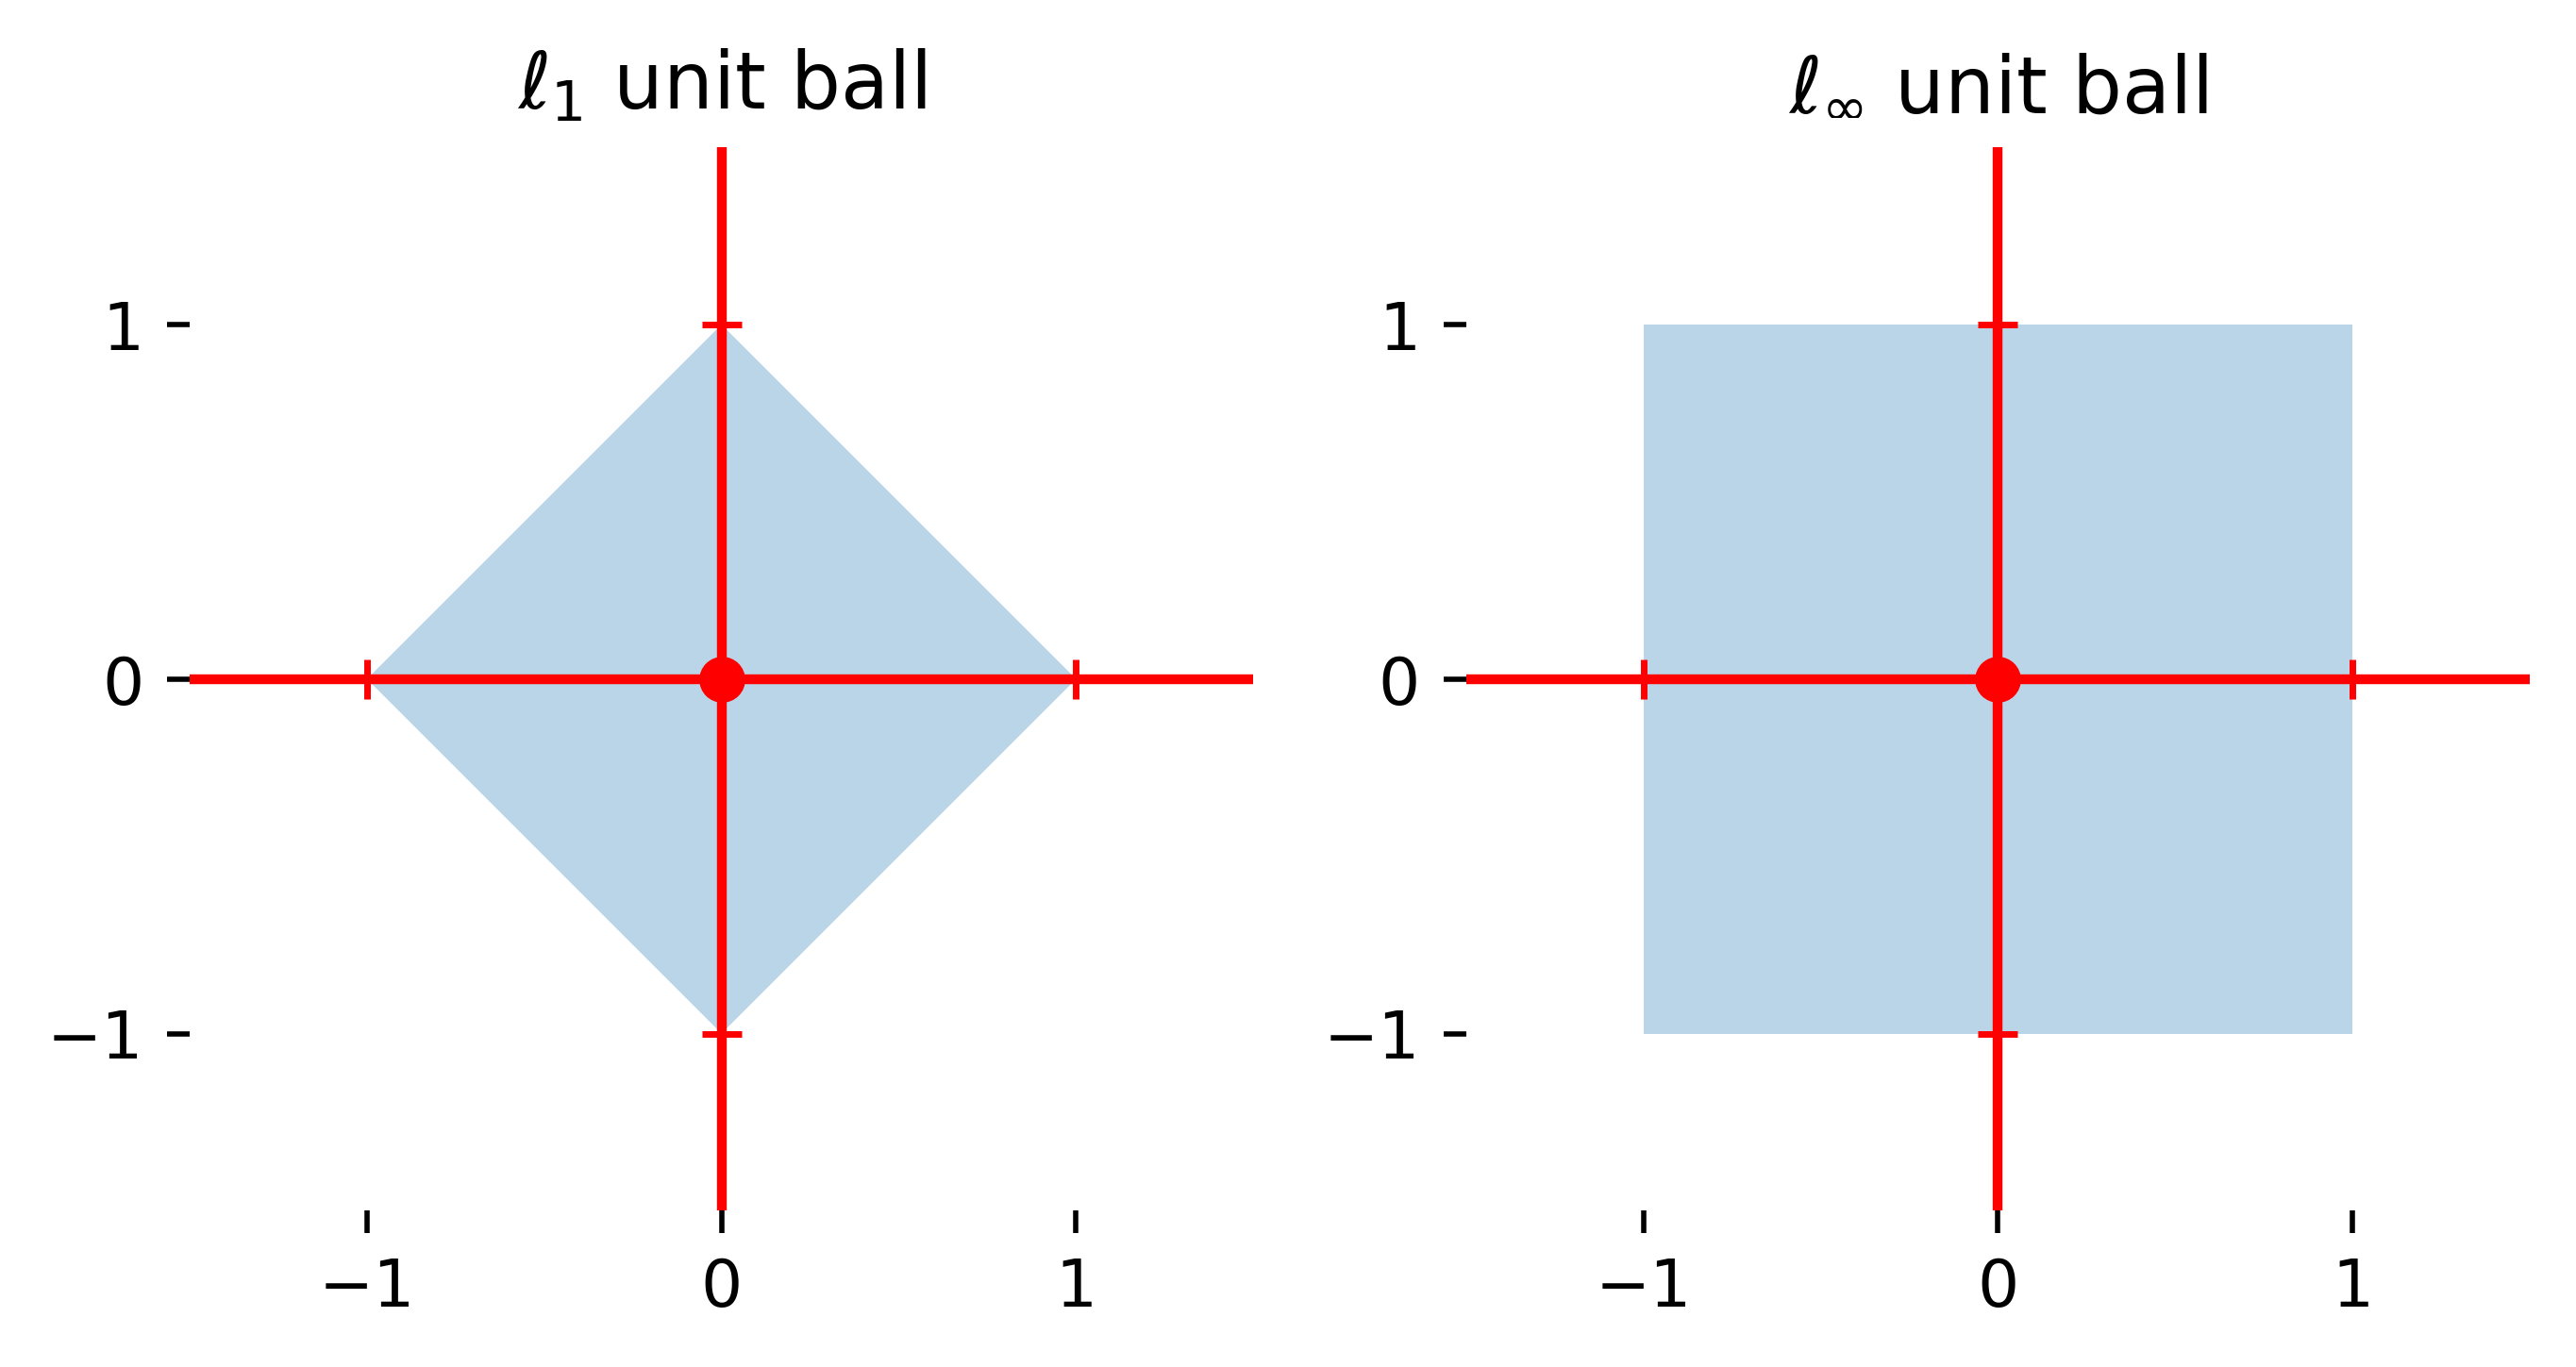
\includegraphics[width=0.6\textwidth]{Images/unit_balls.png}
    \end{figure}

    \item (10 points) Graph $G$ is called a $c$-expander if $\phi_G \geq c$ for some constant $c$. Show that an expander requires $\Omega(\log n)$ distortion to be embedded in $\ell_2$.
\end{enumerate}




\end{problem}
\solution{
\begin{enumerate}[(a)]
  \item The $\ell_1$ embedding of a Tree using the minimum distances will be shown by induction on $|V| = n$. I will write $T_n = (V_n, E_n)$ as the tree with $n$ vertices. Note that the minimum distance on a tree is unique, which will be used in the induction step.
  \begin{itemize}
    \item \underline{Base Case:} $n = 2$
    
    Then $T_2$ is just the path graph, which is immediately embeddable via the mapping $f(v_1) = 0, f(v_2) = 1$, where $f: V_2 \rightarrow \mathbb{R}$. In this case, it holds that dist$(v_1, v_2)$ = $ 1 = \norm{1 - 0}_1 = \norm{f(v_1) - f(v_2)}_1 $, which is the unique minimum distance.
    
    \vspace{5mm}
    \item \underline{Induction Hypothesis:} 

    Next we assume this holds for some $1 < k < n$, that is, $T_k$ is $\ell_1$ embeddable. We will then show this implies $T_{k+1}$ is $\ell_1$ embeddable. 
    
    \vspace{5mm}
    \item \underline{Inductive step:} $n = k+1$
    
    If we consider the subgraph $T_k$ of $T_{k+1}$, we notice these differ by only one leaf vertex - denote this vertex by $v^*$, with edge $\{u^*, v^*\}$ for its parent $u^* \in V^{k}$. By the Induction Hypothesis, we know that $T_k$ is $\ell_1$ embeddable via some mapping $f: V_k \rightarrow \mathbb{R}^{k-1}$. It is then natural to extend this mapping to include $v^*$, so let's define a new function $g: V_{k+1} \rightarrow \mathbb{R}^k$ meant to encapsulate $f$. Define the new function $g$ as follows:
    \[
    g(v)= 
    \begin{cases}
        (f(v), 0)  &,\text{If $v \in V_k$}\\
        (f(u^*), \text{dist}(u^*, v^*)) &,v = v^*
    \end{cases}
    \]
    Note that $g$ does not change distances in $V_{k}$, since if $u, v \in V_k$, then dist$(u, v) = \norm{g(u) - g(v)}_1 = \norm{(f(u), 0) - (f(v), 0)}_1 = \norm{f(u) - f(v)}_1$, which is the unique minimum distance between $u, v$. Next, if $v \in V_k$, we note the following:
    \begin{align*}
    \text{dist}(v^*, v) &\leq \text{dist}(v, u^*) + \text{dist}(u^*, v^*) &\text{(Triangle inequality.)}\\
    &= \norm{f(v) - f(u^*)}_1 + \text{dist}(u^*, v^*) &\text{$T_k$ is $\ell_1$ embeddable.)}\\
    &= \norm{(f(v), 0) - (f(u^*), \text{dist}(u^*, v^*))}_1 &\text{(1-norm definition.)}\\
    &= \norm{g(v) - g(v^*)}_1 &\text{(Definition of $g$.)}
    \end{align*}
    
    Then dist$(v^*, v) \leq \norm{g(v) - g(v^*)}_1$   Note that the minimum distance on a tree graph is unique, therefore dist$(v^*, v) = \norm{g(v) - g(v^*)}_1$ since the inequality in the first step turns into an equality. Thus under the mapping $g$, $T_{k+1}$ is $\ell_1$ embeddable.
    \end{itemize}
    %End part a
    
    %Begin part b
    \item
\end{enumerate}
}

\newpage

\begin{problem}[Image Segmentation using Spectral Clustering (40 points)]
Download {\tt Homework 2 - Spectral Clustering.ipynb} Jupyter Notebook from Canvas and complete the instructions inside. In order to complete this question your choices are to
\begin{enumerate}
    \item Install Jupyter Notebooks locally
    \item Use Google Colab
    \item Use one of the CSIL computers that already has Jupyter Notebooks installed
\end{enumerate}

If you are missing any libraries, install them using `pip install [library]`. You should upload the finished notebook on Gradescope {\bf in the separate programming assignment}.

If you have any questions, come to Konstantinos' office hours or send an email to the instructors.

\end{problem}

\newpage

\end{document}

